\chapter{Formáty uložení řídkých matic}

Formáty uložení řídkých matic obecně ukládají jednotlivé elementy zvlášť a tedy nemusí ukládat ty nulové. To ale přináší řadu nevýhod. Za prvé se musí ukládat informace o souřadicních jednotliých prvcích. Za druhé, ztrácíme možnost přístupu k prvku na libovolných šouřadnicích v čase $\Theta(1)$, protože prvky nemáme přímo indexované podle jejich umístění v řádku a sloupci.

Protože řídké matice můžeme rozdělit do mnoha kategorií a provádět nad nimi mnoho operací, existuje hodně formátů, jak řídkou matici efektivně uložit a pracovat s ní.

\url{http://www.cs.colostate.edu/~mroberts/toolbox/c++/sparseMatrix/sparse_matrix_compression.html}

\subsection{Modifikace řídké matice}

Formáty uložení řídkých matic můžeme také rozdělit podle toho, zda-li je možné do nich přidávat nebo odebírat prvky.

Při násobení matic $C = A \cdot B$ se matice $A$ ani $B$ nemění. V této práci budeme předpokládat, že matice $C$ bude hustá a formáty umožujícími přidávání nebo odebírání prvků nebudou součástí práce. Stejně tak při násobení matice $A$ vektorem $B$ je výsledek $C$ vektor.

\subsection{Uspořádanost řídké matice}

Dalším kritériem pro rozdělení formátů je uspořádanost nenulových prvků v řídké matici. Pro uspořádané prvky bude efektivnější takový formát, který využije určitý vzor. V řídkých maticích takovým vzorem může být například diagonála, nebo blok prvků. Efektivně lze za vzor považovat i prvky v řádku, nebo ve sloupci.

Uspořádáním může být také symetrie matice, kdy nám stačí uložit pouze polovinu matice. Často řídké matice bývají symetrické podle hlavní diagonály.

\section{COO - Coordinate list}

Formát COO, česky seznam souřadnic, je základní formát řídkých matic. Ke~každému nenulovému prvku ukládá jeho souřadnice \texttt{y} a \texttt{x}. Implementovat tento formát můžeme například jako tři pole, jedno s hodnotami prvků, druhé s \texttt{y} souřadnicemi a třetí s \texttt{x} souřadnicemi.

Pro ukázku v tomto formátu uložíme matici o velikosti $n=8$ s $nnz=5$ nenulovými prvky.

\begin{align}
\begin{pmatrix}
	0 & 0 & 0 & 0 & 0 & 0 & 0 & 0 \\
	\boldsymbol{1} & \boldsymbol{2} & 0 & 0 & 0 & 0 & 0 & 0 \\
	0 & 0 & 0 & 0 & 0 & 0 & 0 & 0 \\
	0 & 0 & 0 & 0 & 0 & 0 & 0 & 0 \\
	0 & \boldsymbol{3} & 0 & 0 & 0 & 0 & 0 & 0 \\
	0 & 0 & 0 & 0 & 0 & 0 & 0 & 0 \\
	0 & 0 & 0 & 0 & 0 & \boldsymbol{4} & \boldsymbol{5} & 0 \\
	0 & 0 & 0 & 0 & 0 & 0 & 0 & 0 \\	
\end{pmatrix}
\end{align}

\begin{table}[H]
    \begin{tabular}{r|lllll}
    values[5]   & 1 & 2 & 3 & 4 & 5 \\
    y-coords[5] & 1 & 1 & 4 & 7 & 7 \\
    x-coords[5] & 0 & 1 & 1 & 5 & 6 \\
    \end{tabular}
    \caption{Matice uložená ve formátu COO}
\end{table}

Jak můžeme vidět, délka polí je závislá pouze na $nnz$. Pro velké matice s malým počtem neuspořádaných nenulových prvků je tento formát velmi efektivní. Pokud by bylo prvků velké množství, informace o uložení \texttt{y} nebo \texttt{x} souřadnic by byla často redundatní.

Paměťová náročnost formátu COO je $O(3*nnz)$.

Formát COO je velmi jednoduchý a přímočarý. Při procházení jeho prvků nám stačí jedna iterace přes tři stejně dlouhé pole. Tím je tedy například algoritmus násobení řídké matice ve formátu COO s vektorem velmi jednoduchý:

\begin{algorithm}[H]
	\caption{Násobení matice COO s vektorem}\label{coo-mvm}
	\begin{algorithmic}[1]
		\Procedure{COO-MVM}{COO,V,C}
		\For{\texttt{i$\gets$0\TO COO.nnz}}
			\State \texttt{V.v[COO.r[i]] += COO.v[i] * V.v[COO.c[i]];	}
		\EndFor
		\EndProcedure
	\end{algorithmic}
\end{algorithm}

\label{alg:coo-mmm}
Při násobení dvou matic narazíme na problém. Při této operaci se každý prvek násobí dvakrát. Potřebujeme způsob, jak se v matici vrátit zpátky na určité místo. Takový naivní algoritmus pro násobení dvou COO matic by byl složitý. Museli bychom si pamatovat začátky řádků a neustále kontrolovat, jestli jsme nepřesáhli další řádek. Lepším řešením je dopředu si předpočítat, kde který řádek začíná a končí. Předpočítáme si tedy pole, nazvané $row\_pointers$, o délce $M.height + 1$, obsahující indexy začátků a konců řádek.

Při procháchezní matice se tak v poli s prvky mezi indexy $row\_pointers[i]$ a $row\_pointers[i+1]$ nachází prkvy na řádku $i$. Proto je pole právě o jedna delší než výska matice, abychom mohli určit konec posledního řádku.

\begin{algorithm}[H]
	\caption{Násobení dvou COO matic}\label{coo-mmm}
	\begin{algorithmic}[1]
		\Procedure{COO-MMM}{A,B,C}
		\State \texttt{arp $\gets$ InitArray(A.nnz + 1);}
		\State \texttt{brp $\gets$ InitArray(B.nnz + 1);}
		\For{\texttt{i $\gets$ 0\TO A.nnz}}\Comment{předpočítání prvků v řádcích matice A}
			\State \texttt{arp[A.r[i] + 1] = arp[A.r[i] + 1] + 1;}
		\EndFor
		\For{\texttt{i $\gets$ 0\TO A.height}}
			\State \texttt{arp[i + 1] = arp[i + 1] + arp[i];}
		\EndFor
		\For{\texttt{i $\gets$ 0\TO B.nnz}}\Comment{předpočítání prvků v řádcích matice B}
			\State \texttt{brp[B.r[i] + 1] = brp[B.r[i] + 1] + 1;}
		\EndFor
		\For{\texttt{i $\gets$ 0\TO A.height}}
			\State \texttt{brp[i + 1] = brp[i + 1] + brp[i];}
		\EndFor
		\For{\texttt{i $\gets$ 0\TO A.height}}\Comment{násobení}
			\For{\texttt{ac$\gets$arp[i]\TO arp[i + 1]}}
				\For{\texttt{bc$\gets$brp[A.c[ac]]\TO brp[A.c[ac] + 1]}}
					\State \texttt{C.v[r][A.c[bc]] += A.v[ac] * B.v[bc];}
				\EndFor
			\EndFor
		\EndFor
		\EndProcedure
	\end{algorithmic}
\end{algorithm}

V části s násobením již pole s \texttt{y} souřadnicemi nepotřebujeme. Lepší formát uložení řídkých matic pro násobení by byl takový, který namíto pole s \texttt{y} souřadnicemi obsahuje předpočítané začátky a konce řádků. Takovým formátem je CSR.

%%%%%%%%%%%%%%%%%%%%%%%%%%%%%%%%%%%%%%%%%%%%%%%%%%%%%%%%%%%%%%%%%%%%%%%%%%%%%%
%%%%%%%%%%%%%%%%%%%%%%%%%%%%%%%%%%%%%%%%%%%%%%%%%%%%%%%%%%%%%%%%%%%%%%%%%%%%%%
%%%%%%%%%%%%%%%%%%%%%%%%%%%%%%%%%%%%%%%%%%%%%%%%%%%%%%%%%%%%%%%%%%%%%%%%%%%%%%
%%%%%%%%%%%%%%%%%%%%%%%%%%%%%%%%%%%%%%%%%%%%%%%%%%%%%%%%%%%%%%%%%%%%%%%%%%%%%%
%%%%%%%%%%%%%%%%%%%%%%%%%%%%%%%%%%%%%%%%%%%%%%%%%%%%%%%%%%%%%%%%%%%%%%%%%%%%%%
%%%%%%%%%%%%%%%%%%%%%%%%%%%%%%%%%%%%%%%%%%%%%%%%%%%%%%%%%%%%%%%%%%%%%%%%%%%%%%

\section{CSR - Compressed sparse row}

Problém efektivnosti formátu COO pro větší množství prvků řeší formát CSR, česky komprimované řídké řádky. Formát CSR obsahuje pole $row\_pointers$, které ukládá informace o tom, kolik se v daném řádku nachází prvků, tedy přesně to, co jsme si přespočítali v algoritmu \ref{coo-mmm}. K poli s hodnotami je další pole $col\_indicies$, přiřazující ke každému prvku informaci o sloupci.

\begin{figure}[H]\centering
	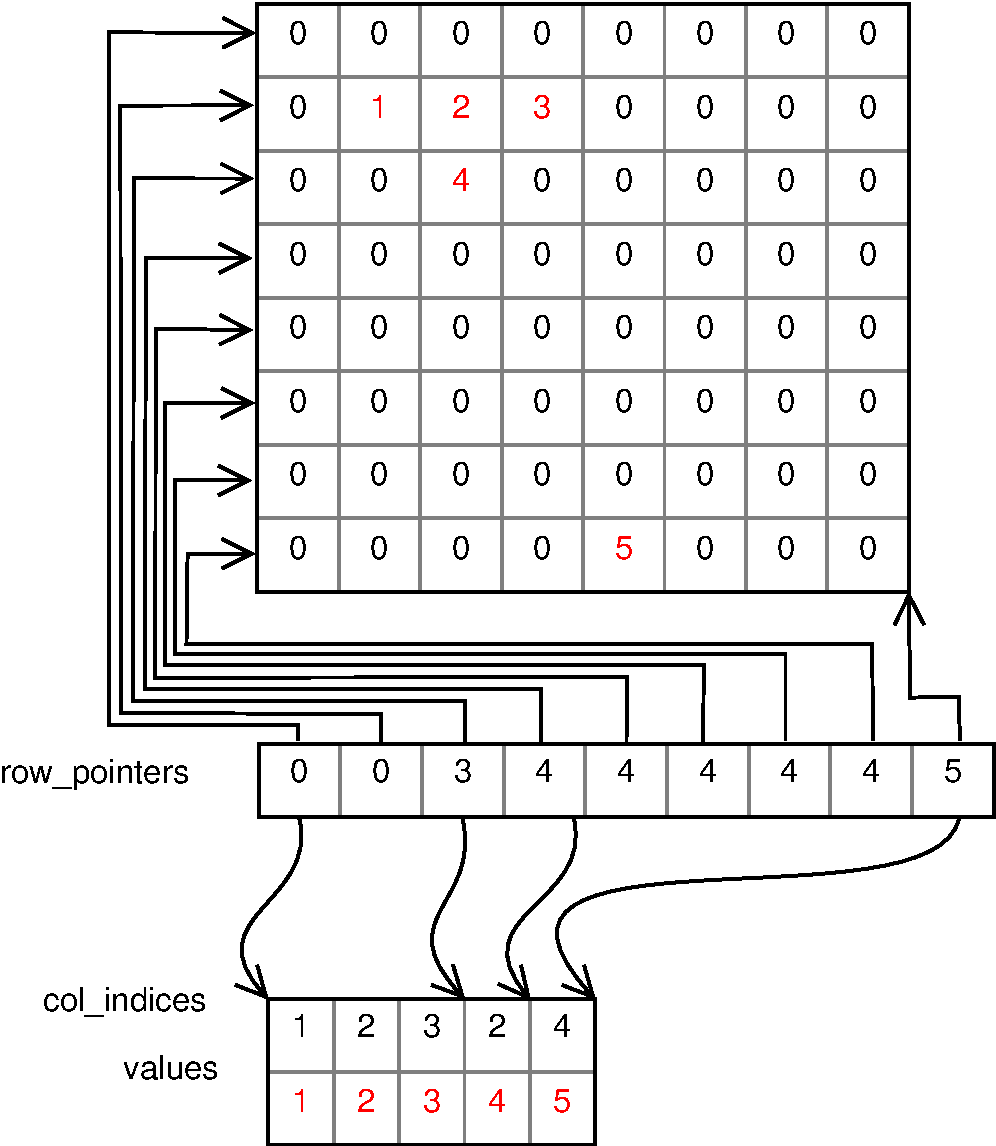
\includegraphics[width=\textwidth]{./images/csr/csr}
	\caption{Matice uložená ve formátu CSR}
	\label{fig:CSR}
\end{figure}

Jak je vidět z ilustrace \ref{fig:CSR}, řádek s více prvky je uložen efektivně. Díky prázdným řádkům se nezdá pole $row\_pointers$ rozumně využité.

Při násobení matice CSR s vektorem potřebujeme o jeden for cyklus více než v případě násobení matice COO s vektorem. Důvodem je ztráta informace o řádku prvku.

\begin{algorithm}[H]
	\caption{Násobení matice CSR s vektorem}\label{csr-mvm}
	\begin{algorithmic}[1]
		\Procedure{CSR-MVM}{CSR,V,C}
		\For{\texttt{i $\gets$ 0 \TO CSR.h}}
			\For{\texttt{ci $\gets$ CSR.rp[i]\TO CSR.rp[i + 1]}}
				\State \texttt{C.v[r] += CSR.v[ci] * V.v[A.ci[ci]];}
			\EndFor
		\EndFor
		\EndProcedure
	\end{algorithmic}
\end{algorithm}

Násobení dvou CSR matic je stejné jak v případě násobení dvou COO matic \ref{fig:CSR}. Jediný rozdíl je, že předpočíné začátky a konce řádků jsou součástí formátu.

\label{alg:csr-mmm}
\begin{algorithm}[H]
	\caption{Násobení dvou CSR matic}\label{csr-mmm}
	\begin{algorithmic}[1]
		\Procedure{CSR-MMM}{A,B,C}
		\For{\texttt{i $\gets$ 0\TO A.height}}\Comment{násobení}
			\For{\texttt{ac $\gets$ A.rp[i]\TO A.rp[i + 1]}}
				\For{\texttt{bc $\gets$ B.rp[A.ci[ac]]\TO B.rp[A.ci[ac] + 1]}}
					\State \texttt{C.v[r][B.ci[bc]] += A.v[ac] * B.v[bc];}
				\EndFor
			\EndFor
		\EndFor
		\EndProcedure
	\end{algorithmic}
\end{algorithm}

Existuje varianta tohoto formátu, nazvaná CSC - compressed sparse columns, která místo ukládání řádku ukládá sloupce.

\section{BSR - Block Sparse Row}

Jako formát CSR využívá uložení prvků v řádku, formát BSR ještě navíc detekuje a ukládá prvky v blocích.

Protože při násobení matic násobíme každý prvek dvakrát, bylo by dobré tyto dvě operace provést co nejdříve, abychom při druhém znovunačtení prvku mohli sáhnout pro prvek do cache. Pokud jsou prkvy procházené po menších blocích, dostaneme se k prvku podruhé dříve, než jej z cache přemaže jiný prvek.

Matici $A$ ve formátu BSR uklákáme, velice podobně jako u formátu CSR, pomocí tří polí. Je potřeba i jedna proměnná, která uchovává velikost bloku. Tuto proměnnou nazveme $block\_size$. Matici rozdělíme do bloků Pole $col\_indices$ označuje sloupec, ve kterém se blok nachází. Sloupcem rozumíme $A.width / A.block\_size$.

\begin{figure}[H]\centering
	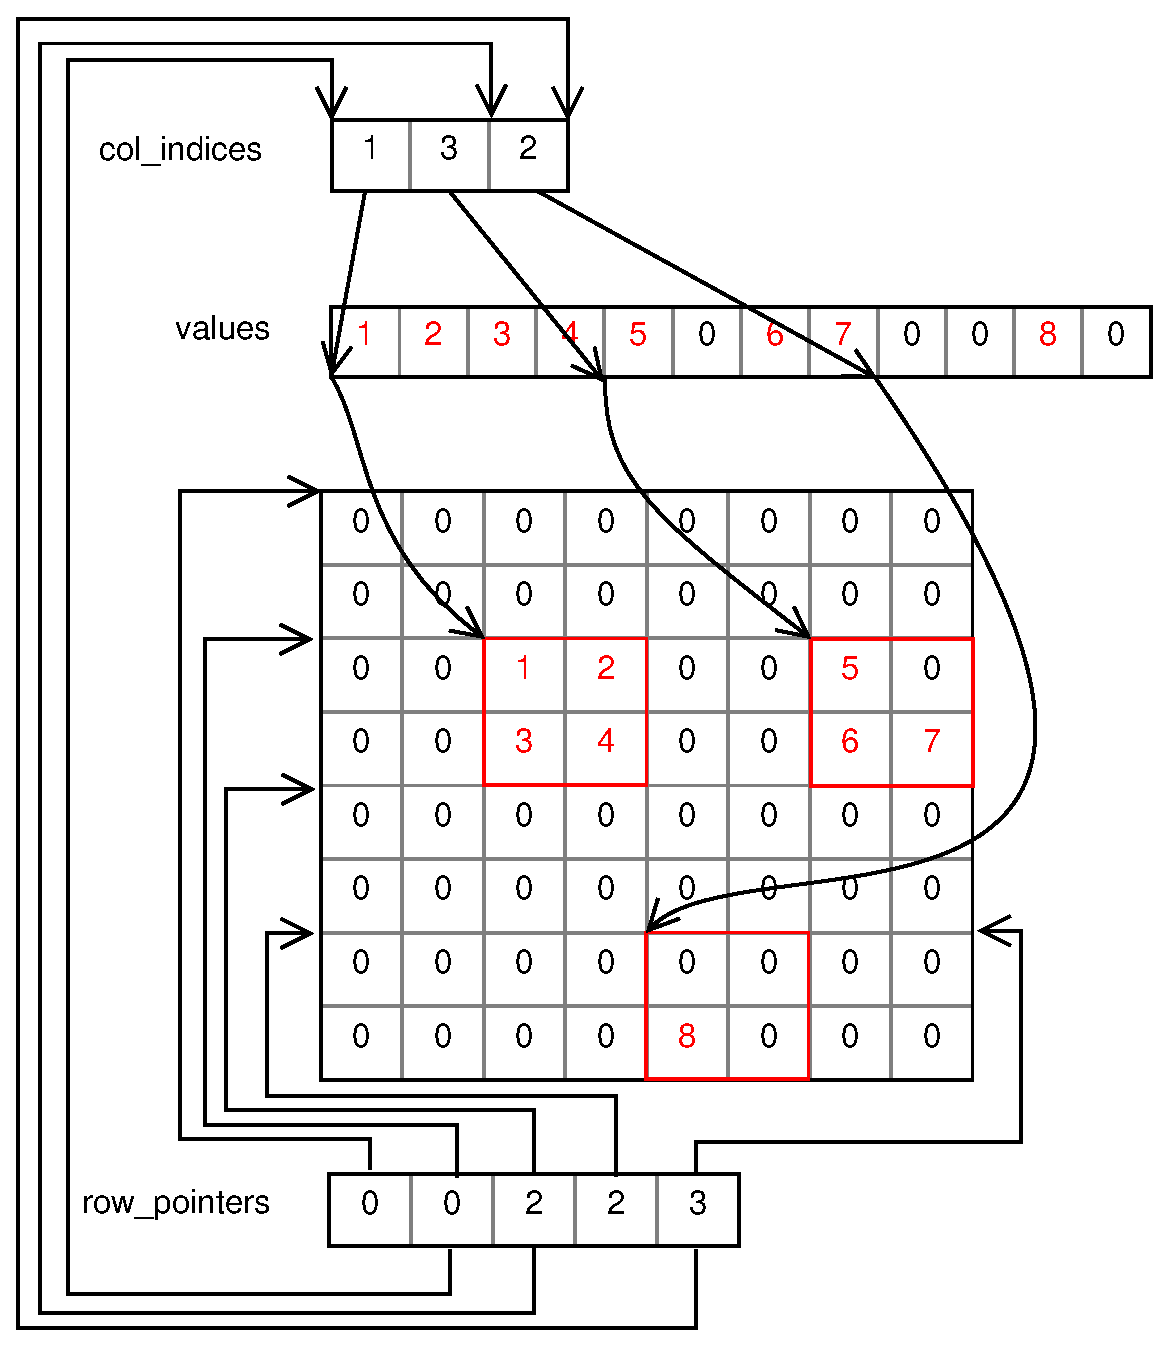
\includegraphics[width=\textwidth]{./images/bsr/bsr}
	\caption{Matice uložená ve formátu BSR}
	\label{fig:BSR}
\end{figure}

Uložení matice ve formátu BSR ilustruje obrázek \ref{fig:BSR}. Pole $row\_pointers$ obsahuje informace o tom, na kterém řádku je kolik bloků. Na řádku $i$ je $row\_pointers[i+1] - row\_pointers[i]$ bloků. Ve kterém sloupci se blok prvků nachází udává pole $col\_indices$. První blok z řádku $i$ je ve sloupci $col\_indices[row\_pointers[i]]$ a poslední blok je ve sloupci $col\_indices[row\_pointers[i+1]]$. Pole $values$ obsahuje prvky v blocích, včetně nulových prvků.

Pokud vezmeme algoritmus násobení dvou CSR matic respektive CSR matice s vektorem, jen místo prvků násobíme bloky, vznikne nám algoritmus pro násobení dvou BSR matric respektive BSR matice s vektorem. Za povšimnutí stojí větší počet for cyklů s menším rozsahem iterace než u CSR. To nám v nejvnitřnejších cyklech dovoluje lépe využívat cache. Jedná se tedy o přístup podobný optimalizační technice loop tiling.

\label{alg:bsr-mvm}
\begin{algorithm}[H]
	\caption{Násobení matice BSR s vektorem}\label{bsr-mvm}
	\begin{algorithmic}[1]
		\Procedure{BSR-MVM}{A,B,C}
		\State \texttt{bs $\gets$ A.block\_size;}
		\For{\texttt{i $\gets$ 0\TO A.height / bs}}
			\For{\texttt{ac $\gets$ A.rp[i]\TO A.rp[i + 1]}}
				\For{\texttt{l $\gets$ 0 \TO A.bs}}\Comment{násobení bloku}
					\For{\texttt{m $\gets$ 0\TO bs}}
						\State \texttt{C.v[(i * bs) + l] += A.v[ac * (bs * bs) + (l * bs) + m] * B.v[A.ci[ac] * bs + m];}
					\EndFor
				\EndFor
			\EndFor
		\EndFor
		\EndProcedure
	\end{algorithmic}
\end{algorithm}

\label{alg:bsr-mmm}
\begin{algorithm}[H]
	\caption{Násobení dvou BSR matic}\label{bsr-mmm}
	\begin{algorithmic}[1]
		\Procedure{BSR-MMM}{A,B,C}
		\State \texttt{bs $\gets$ A.block\_size;}
		\For{\texttt{i $\gets$ 0\TO A.height / bs}}
			\For{\texttt{ac $\gets$ A.rp[i]\TO A.rp[i+1]}}
				\For{\texttt{bc $\gets$ B.rp[A.ci[ac]]\TO B.rp[A.ci[ac]+1]}}
					\For{\texttt{l $\gets$ 0\TO A.bs}}\Comment{násobení bloku}
						\For{\texttt{m $\gets$ 0\TO bs}}
							\For{\texttt{n $\gets$ 0\TO bs}}
								\State \texttt{C.v[(i * bs) + l][(B.ci[bc] * bs) + m] += A.v[ac * (bs * bs) + (l * bs) + n] * B.v[bc * (bs * bs) + (n * bs) + m];}
							\EndFor
						\EndFor
					\EndFor
				\EndFor
			\EndFor
		\EndFor
		\EndProcedure
	\end{algorithmic}
\end{algorithm}

\url{http://docs.scipy.org/doc/scipy-0.13.0/reference/generated/scipy.sparse.bsr_matrix.html}
\url{https://software.intel.com/sites/products/documentation/doclib/mkl_sa/11/mklman/GUID-9FCEB1C4-670D-4738-81D2-F378013412B0.htm}

\section{Quadtree}

Předchozí popsáné formáty uložení řídkých matic jsou velmi přímočaré. Neumožnují rekurzivní přístup, který je pro velké matice vhodnější. Tento problém řeší formát Quadtree \cite{JA_SNA_08_QUAD}. Jedná se o matici uloženou v 4-árním stromě.

Tento formát dělí matici na čtvrtiny do té doby, než se dosáhne velikosti podmatice $sm\_size$. Pokud je celá čtvrtina prázdná, je uzel označen jako prázdný, označen $E$. Pokud obsahuje nějaké prvky, je list označen jako hustý, $D$. Vnitřní uzly jsou označeny jako smíšené, tedy $M$.

\begin{figure}[H]\centering
	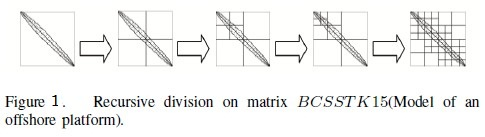
\includegraphics[width=\textwidth]{./images/quadtree_sourceforge/figure4}
	\caption{Rozdělení matice}
	\label{fig:BSR}
\end{figure}

\begin{figure}[H]\centering
	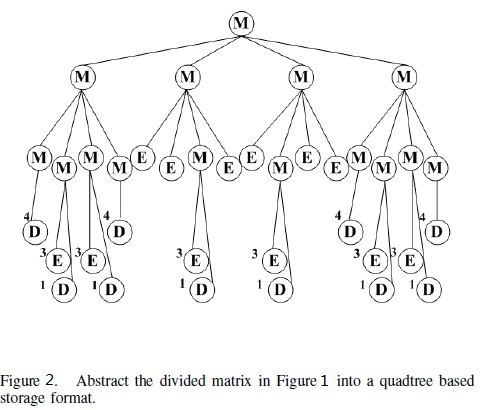
\includegraphics[width=\textwidth]{./images/quadtree_sourceforge/figure5}
	\caption{Strom matice uložené ve formátu Quadtree}
	\label{fig:BSR}
\end{figure}

\url{http://quardtree.sourceforge.net/}

Algoritmy pro práci s formátem Quadtree budou ukázány v kapitole o obecnějším formátě \ref{katchapter}.

\section{?}

TODO: tady jsem chtel spocictat kdy  se vyplati mit ridkou matici, ale lepsi bude tabulka. Pokud například uložíme matici o rozměrech 100x100 v dvojté přestnosti, bude zabírat \texttt{M x N x sizeof(double) = 100 x 100 x 8 = 80000B = 80kB}. Pokud zvolíme řídký formát matice, kde ke každému elementu uložíme i jeho x a y souřadnici, tak do 80kB uložíme \texttt{80000 / (sizeof(int)+sizeof(int)+sizeof(double)) = 80000/16= 5000} elementů. Pokud matice obsahuje více jak 50  \% nulových elementů, vyplatí se nám ji uložit do řídkého formátu.

%-----------------------------------------------------------------------------

\label{katchapter}
\chapter{Modifikace formátu quadtree}

Protože formát Quadtree je 4-ární strom, jeho výška při reprezentaci matice o velikosti $n$ a při velikosti podmatice $sm\_size$ je:

% n=1024 ss=128 height=3
%

\label{quadtreeheight}
\begin{align}
\Bigg\lceil\log_{4}\frac{n^2}{sm\_size^2}\Bigg\rceil
\end{align}

Například pro matici o velikosti $n=16384$ s velikostí bloku $sm\_size=128$ je výška stromu $7$.

\section{KAT - k-ary tree matrix}

V této práci navrhneme místo 4-árního stromu obecný $k$-ární strom. Výška stromu se tím sníží. Pro předchozí příklad by tedy pro 32-ární strom byla výška pouze $3$. Tento formát nazveme \texttt{k-ary tree matrix} se zkratkou KAT. Pro přehlednost nebudeme uvádět $k$, ale $KAT.n = sqrt(k)$. Formát Quadtree můžeme prohlásit za matici KAT s $KAT.n = 2$.

\section{Typy listů}

Formát Quadtree definovaný v (cituj) označí všechny nenulové listy jako husté a ukládá je v COO formátu. KAT matice obasahuje proměnnou $KAT.dense\_treshold$, která udává maximální počet prvků, aby se s listem pracovalo některým z řídkých formátů, tedy COO, CSR, BSR. Při překročení této hranice je list uložen ve formátu husté matice, tedy bude obsahovat i nulové prvky.

\section{Tvoření stromu}

Pro každý prvek procházíme strom a hledáme správný list. Protože výška stromu je daná třemy parametry, tedy velikostí matice $n$, velikostí podmatice $sm\_size$ a počtu větvení uzlu $k$, čelíme problému, nejefektivnější využití bude, pokud je $n$ bezezbytku dělitelné $k * sm_size$. Pokud toto neplatí, rodiče listů budou mít část synů nevyužitých i při uložení husté matice.

\label{alg:kat-create}
\begin{algorithm}[H]
	\caption{Vyhledání listu pro KAT matici}\label{kat-create}
	\begin{algorithmic}[1]
		\Procedure{KAT-getNode}{KAT, y, x}
		\State \texttt{tmpNode $\gets$ KAT.root;}
		\State \texttt{blockY $\gets$ 0;}\Comment{výřez matice}
		\State \texttt{blockX $\gets$ 0;}
		\State \texttt{blockS $\gets$ KAT.sm\_size;}
		\\\Comment{až do předposledního vnitřního uzlu traverzujeme podle velikosti KAT.n}
		\While{\texttt{blockS > (KAT.n * KAT.sm\_size)}}
			\State \texttt{nodeY $\gets$ (y - blockY) / (blockS / KAT.n);}
			\State \texttt{nodeX $\gets$ (x - blockX) / (blockS / KAT.n);}
			\State \texttt{tmpNode $\gets$ tmpNode.childs[nodeY][nodeX];}
			\State \texttt{blockY += nodeY * (blockS / KAT.n);}
			\State \texttt{blockX += nodeX * (blockS / KAT.n);}
			\State \texttt{blockS /= KAT.n;}
		\EndWhile
		\\\Comment{do posledního vnitnřního uzlu traverzujeme podle velikosti KAT.sm\_size}
		\State \texttt{nodeY $\gets$ (y - blockY) / KAT.sm\_size;}
		\State \texttt{nodeX $\gets$ (x - blockX) / KAT.sm\_size;}
		\State \texttt{tmpNode $\gets$ tmpNode.childs[nodeY][nodeX];} 	
		\\\Comment{nyní je tmpNode list}
		\State \texttt{tmpNode.x $\gets$ $\lfloor$y / KAT.sm\_size$\rfloor$ * KAT.sm\_size ;}
		\State \texttt{tmpNode.x $\gets$ $\lfloor$x / KAT.sm\_size$\rfloor$ * KAT.sm\_size ;}
		\State \texttt{return tmpNode;}
		\EndProcedure
	\end{algorithmic}
\end{algorithm}

\section{Násobení}

Pro násobení budeme používat algoritmus rekurzivního násobení popsaného v \ref{RecMul}. Popsaný algormus dělí matice na čtvrtiny, jde tedy aplikovat na formát Quadtree. Při násobení matice uložené v $k$-árním stromě budeme násobit matici podmatic o velikosti $k$:

\label{alg:kat-mvm}
\begin{algorithm}[H]
	\caption{Násobení matice KAT s vektorem}\label{kat-mvm}
	\begin{algorithmic}[1]
		\Procedure{KAT-MVM}{KAT, KAT\_node, VB, VC}
		\For{\texttt{i $\gets$ 0\TO KAT.n}}
			\For{\texttt{j $\gets$ 0\TO KAT.n}}
				\If{\texttt{KAT\_node.childs[i][j] $\neq$ NIL}}
					\If{\texttt{KAT\_node.childs[i][j].type = "submatrix"}}
						\State \texttt{multiplyNode(KAT\_node.childs[i][j], VB, VC);}
						\State \texttt{coninue;}
					\EndIf
					\If{\texttt{KAT\_node.childs[i][j].type = "inner"}}
						\State \texttt{KAT-MVM(KAT,KAT\_node.childs[i][j], VB, VC);}
						\State \texttt{coninue;}
					\EndIf
				\EndIf
			\EndFor
		\EndFor
		\EndProcedure
	\end{algorithmic}
\end{algorithm}

\label{alg:kat-mmm}
\begin{algorithm}[H]
	\caption{Násobení dvou KAT matic}\label{kat-mmm}
	\begin{algorithmic}[1]
		\Procedure{KAT-MMM}{KATa, KATa\_node, KATb, KATb\_node, C}
		\For{\texttt{i $\gets$ 0\TO KAT.n}}
			\For{\texttt{j $\gets$ 0\TO KAT.n}}
				\For{\texttt{k $\gets$ 0\TO KAT.n}}
					\If{\texttt{KATa\_node.childs[i][k] $\neq$ NIL and KATb\_node.childs[k][j] $\neq$ NIL}}
						\If{\texttt{KAT\_node.childs[i][j].type = "submatrix"}}
							\State \texttt{multiplyNode(KAT\_node.childs[i][j], KAT\_node.childs[i][j], VC);}
							\State \texttt{coninue;}
						\EndIf
						\If{\texttt{KAT\_node.childs[i][k].type = "inner"}}
							\State \texttt{KAT-MMM(KATa,KATa\_node.childs[i][k], KATb,KATb\_node.childs[k][j] C);}
							\State \texttt{coninue;}
						\EndIf
					\EndIf
				\EndFor
			\EndFor
		\EndFor
		\EndProcedure
	\end{algorithmic}
\end{algorithm}

je to samostatnej bod v zadani tak by to mohla byt cela chapter

TODO: popsat nevyhody quadtree a obrazkama ukazat jak to udelat lip

neco jako quadtree loop unrolling
